\chapter{Rezultati} % Main chapter title
\label{Chapter6}

Za svaki od tri prethodno opisana metoda binarne klasifikacije trenirano je po 398 modela na celom trening skupu koji su kasnije ujedinjeni u 3 prediktora za predviđanje funkcije proteina. Implementiran je još jedan jednostovaniji klasifikator koji je poslužio kao osnovna metoda za poređenje rezultata. U pitanju je naivni klasifikator koji svakom čvoru dodeljuje vrednost koja odgovara njegovoj frekvenciji pojavljivanja u trening skupu i tako formirani graf pridružuje svakom test primeru \cite{doktJK}. 

Naivni klasifikator je testiran na istom test skupu kao i 3 prediktora pri čemu su određene prosečne vrednosti za 5 mera kvaliteta modela i to $f_1$-mera, tačnost, preciznost, odziv i površina ispod ROC krive. Prilikom svakog testiranja računata je prosečna vrednost svake mere kvaliteta i to na nivou pojedinačnih organizama, kao i na nivou celog skupa. 

Sa slike \ref{fig:f1scores} se može videti da je svaki od tri prediktora bolji od naivnog klasifikatora prema $f1$-meri. Pored toga, sva 3 prediktora na celom skupu imaju približnu $f1$-meru. Nešto slabiji rezultat metode potpornih vektora mogu se objasniti primenom analize glavnih komponenti na trening skup čime je izgubljen deo informacija. 


Poređenje tačnosti, prikazano na slici \ref{fig:accscores}, pokazuje da svi modeli imaju sličnu tačnost, što može biti posledica nebalansiranog skupa podataka jer je visoka tačnost postignuta zbog velikog broja ispravno klasifikovanih negativnih instanci, a pošto je skup nebalansiran u korist negativne klase, većina instanci je dobro klasifikovana. Prema preciznosti (slika \ref{fig:prescores}) se ističu modeli metode slučajne šume, dok su prema odzivu (slika \ref{fig:recscores}) bliski klasifikatori metode potpornih vektora i logističke regresije. Sa svih grafika na slici \ref{fig:eval} vidi se da su rezultati konzistentni za sve organizme. Na primer, predviđanje funkcija proteina čoveka ne daje bolje rezultate nego predviđanje funkcija proteina za ostale organizme.


U tabelama \ref{tab: rfF1}, \ref{tab: lrF1} i \ref{tab: svmF1} za 20 najboljih\footnote{Najboljih prema vrednosti za $f1$-meru.} pojedinačnih klasifikatora za svaku upotrebljenu metodu binarne klasifikacije prikazane su vrednosti za $f_1$-meru, tačnost, preciznost, odziv, površinu ispod krive, kao i nivo na kom se čvor nalazi u grafu, broj i procenat pojavljivanja funkcije u trening skupu. Pored toga, prikazan je i broj pojavljivanja u trening skupu za svaku funkciju, kao i udeo broja pojavljivanja funkcije u celom trening skupu. Vrednosti za sve klasifikatore prikazane su na adresi \url{http://poincare.matf.bg.ac.rs/~anja_bukurov/master/}.


\begin{figure}[H]
	\begin{subfigure}{0.9\textwidth}
		\centering
		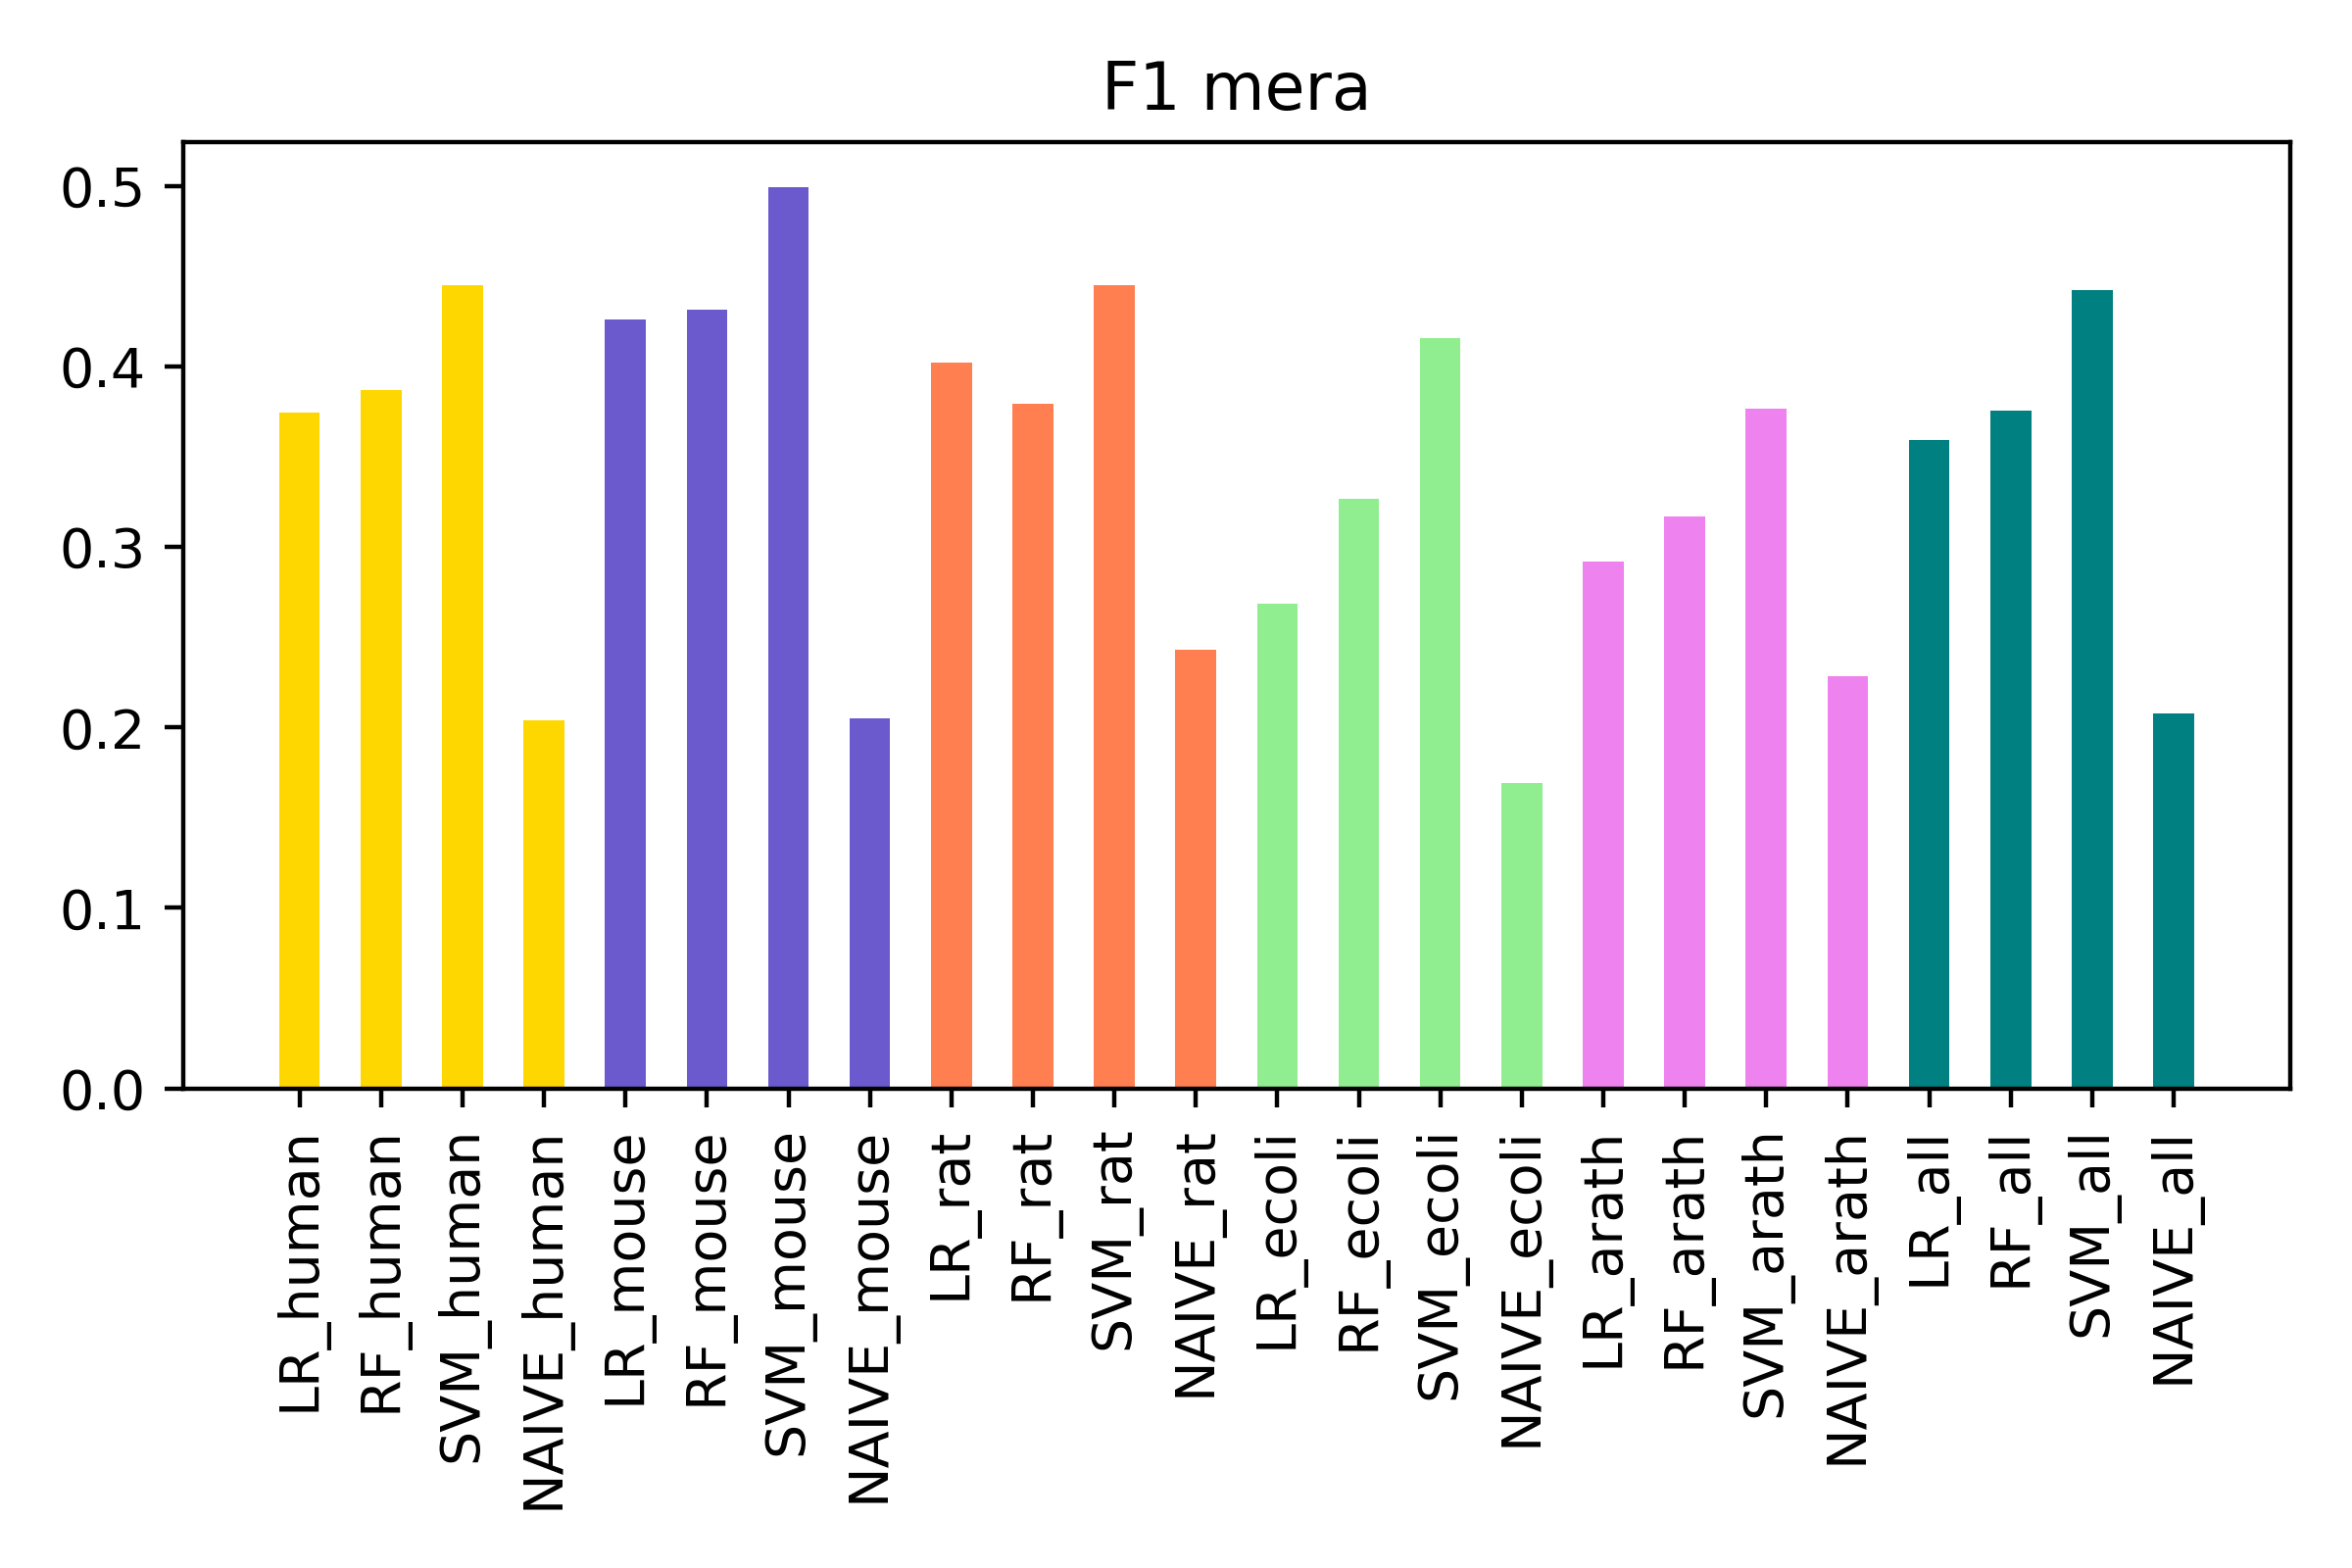
\includegraphics[width=\textwidth]{Figures/f1_poredjenje.png}
		\caption{Poređenje prediktora i naivnog klasifikatora prema f1-meri.}
		\label{fig:f1scores}
	\end{subfigure}

	\begin{subfigure}{0.5\textwidth}
		\centering
		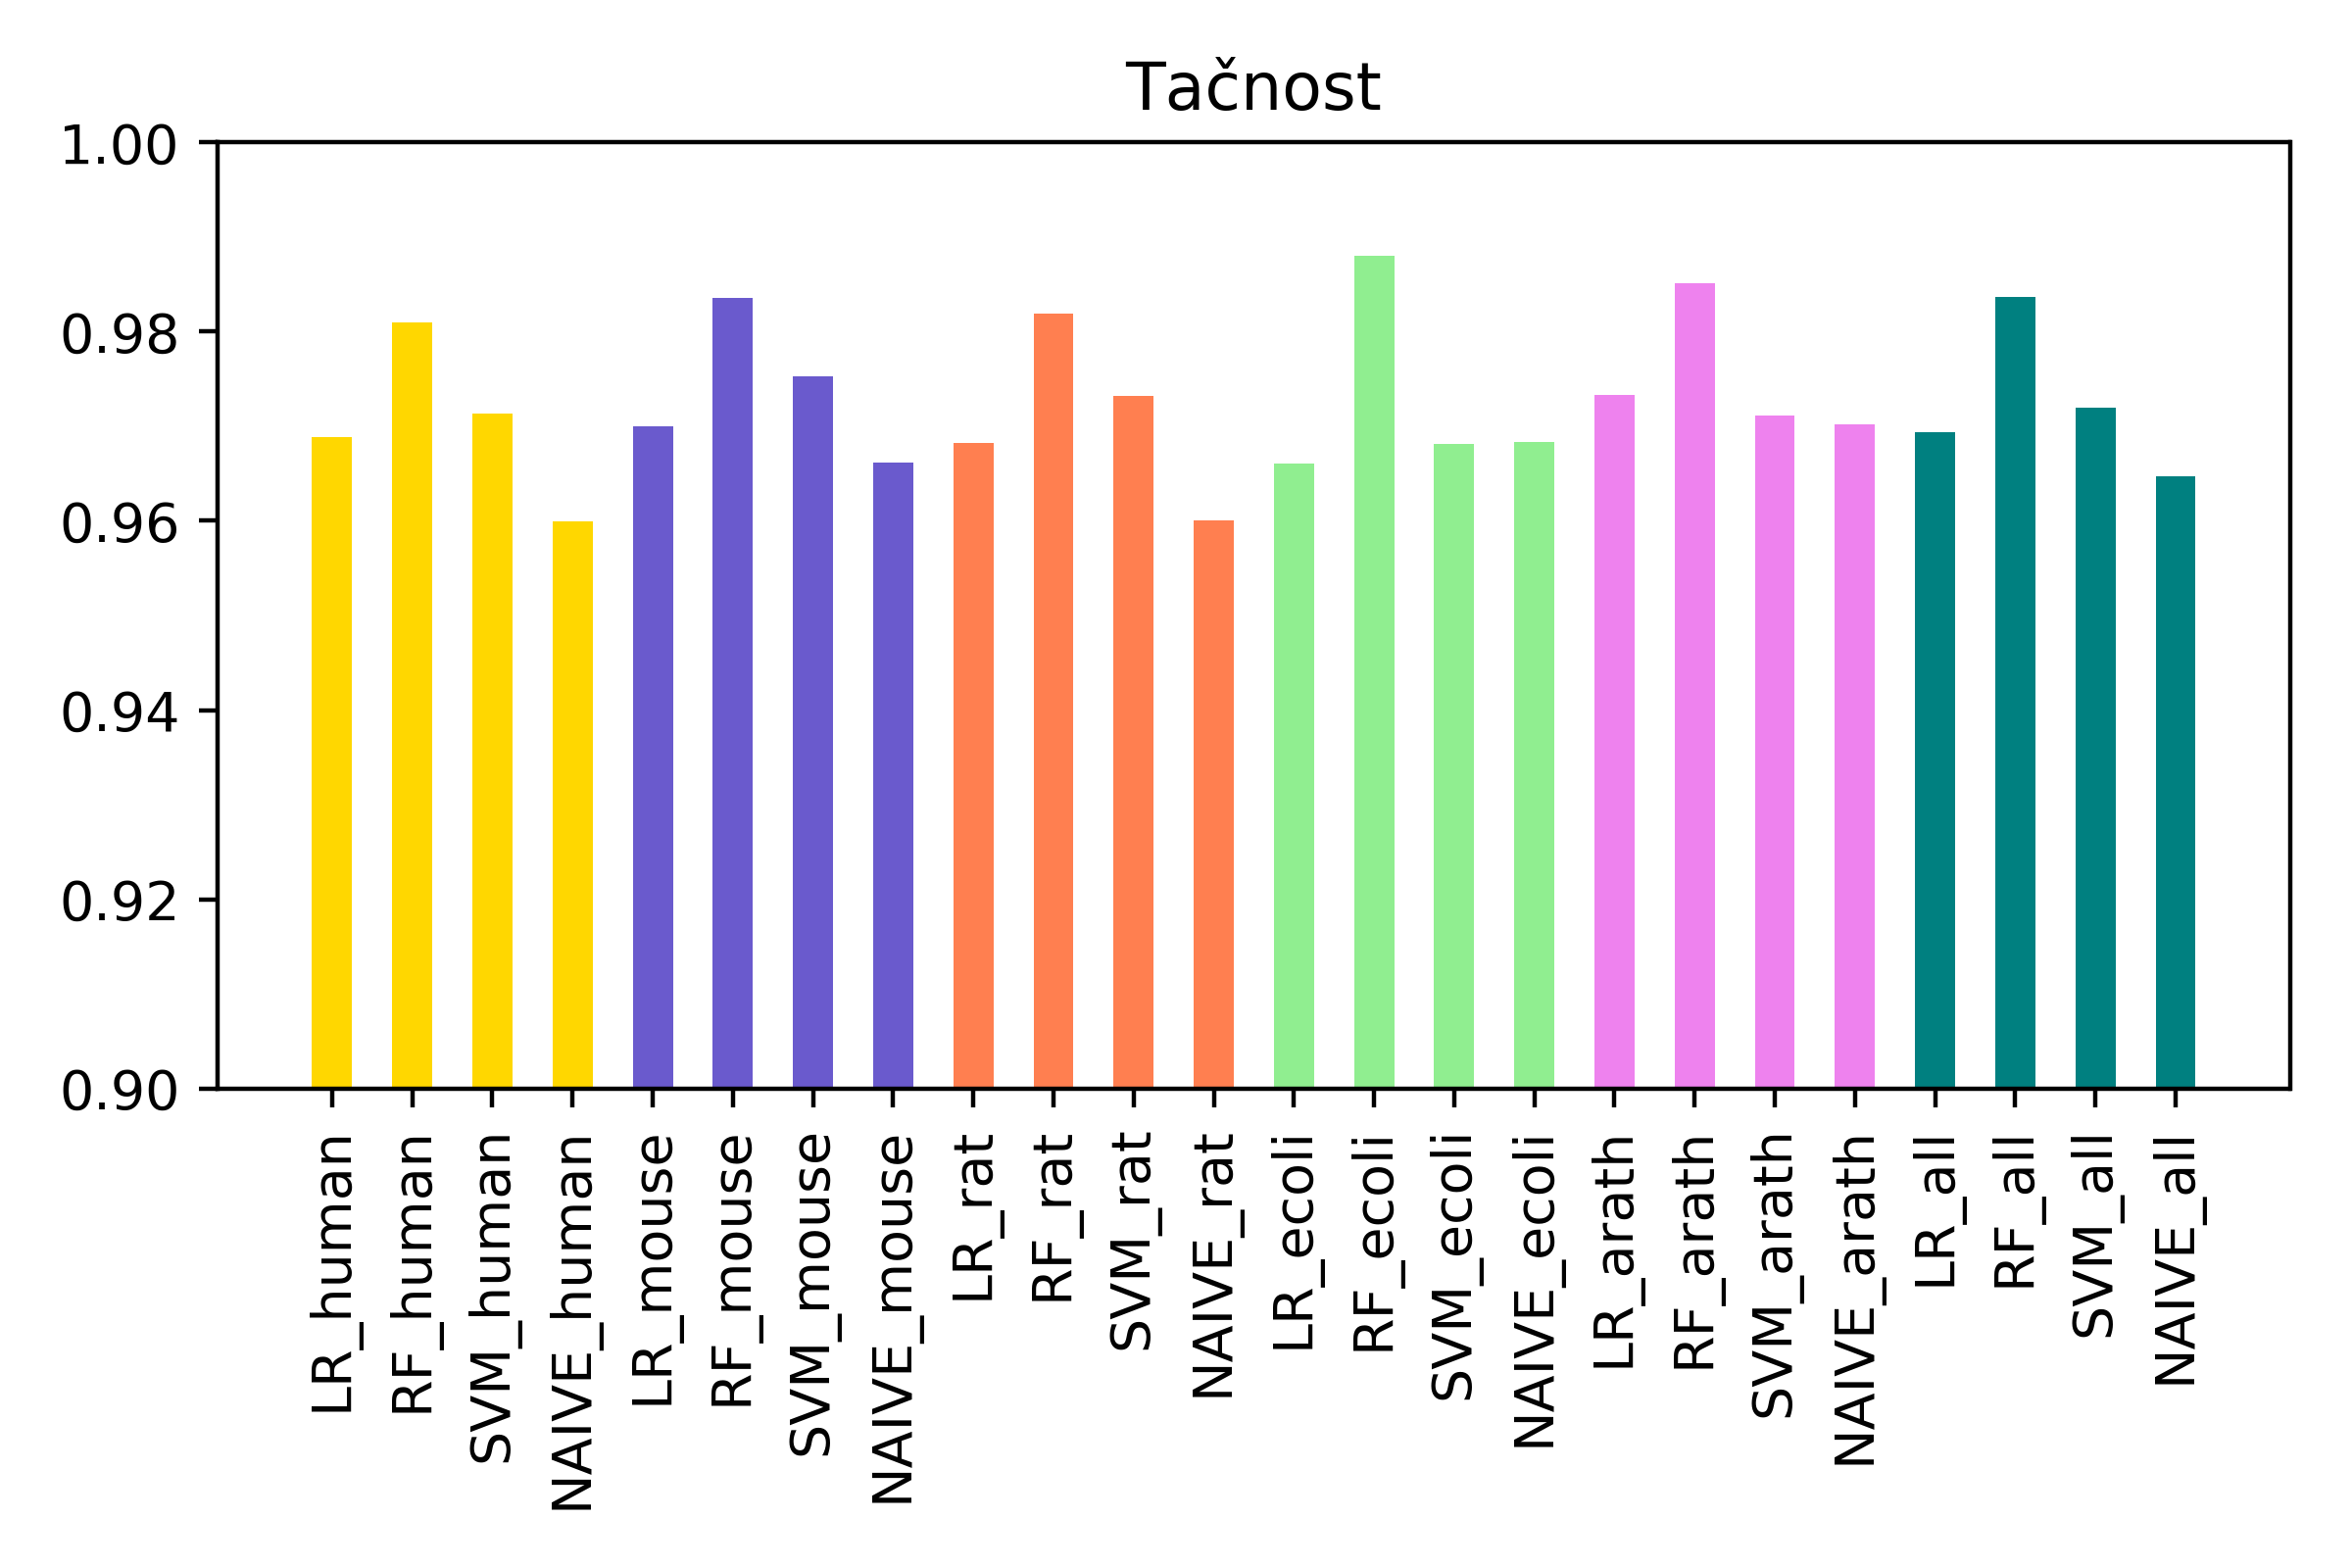
\includegraphics[width=\textwidth]{Figures/acc_poredjenje.png}
		\caption{Poređenje prema tačnosti. }
		\label{fig:accscores}
	\end{subfigure}
	\begin{subfigure}{0.5\textwidth}
		\centering
		% include second image
		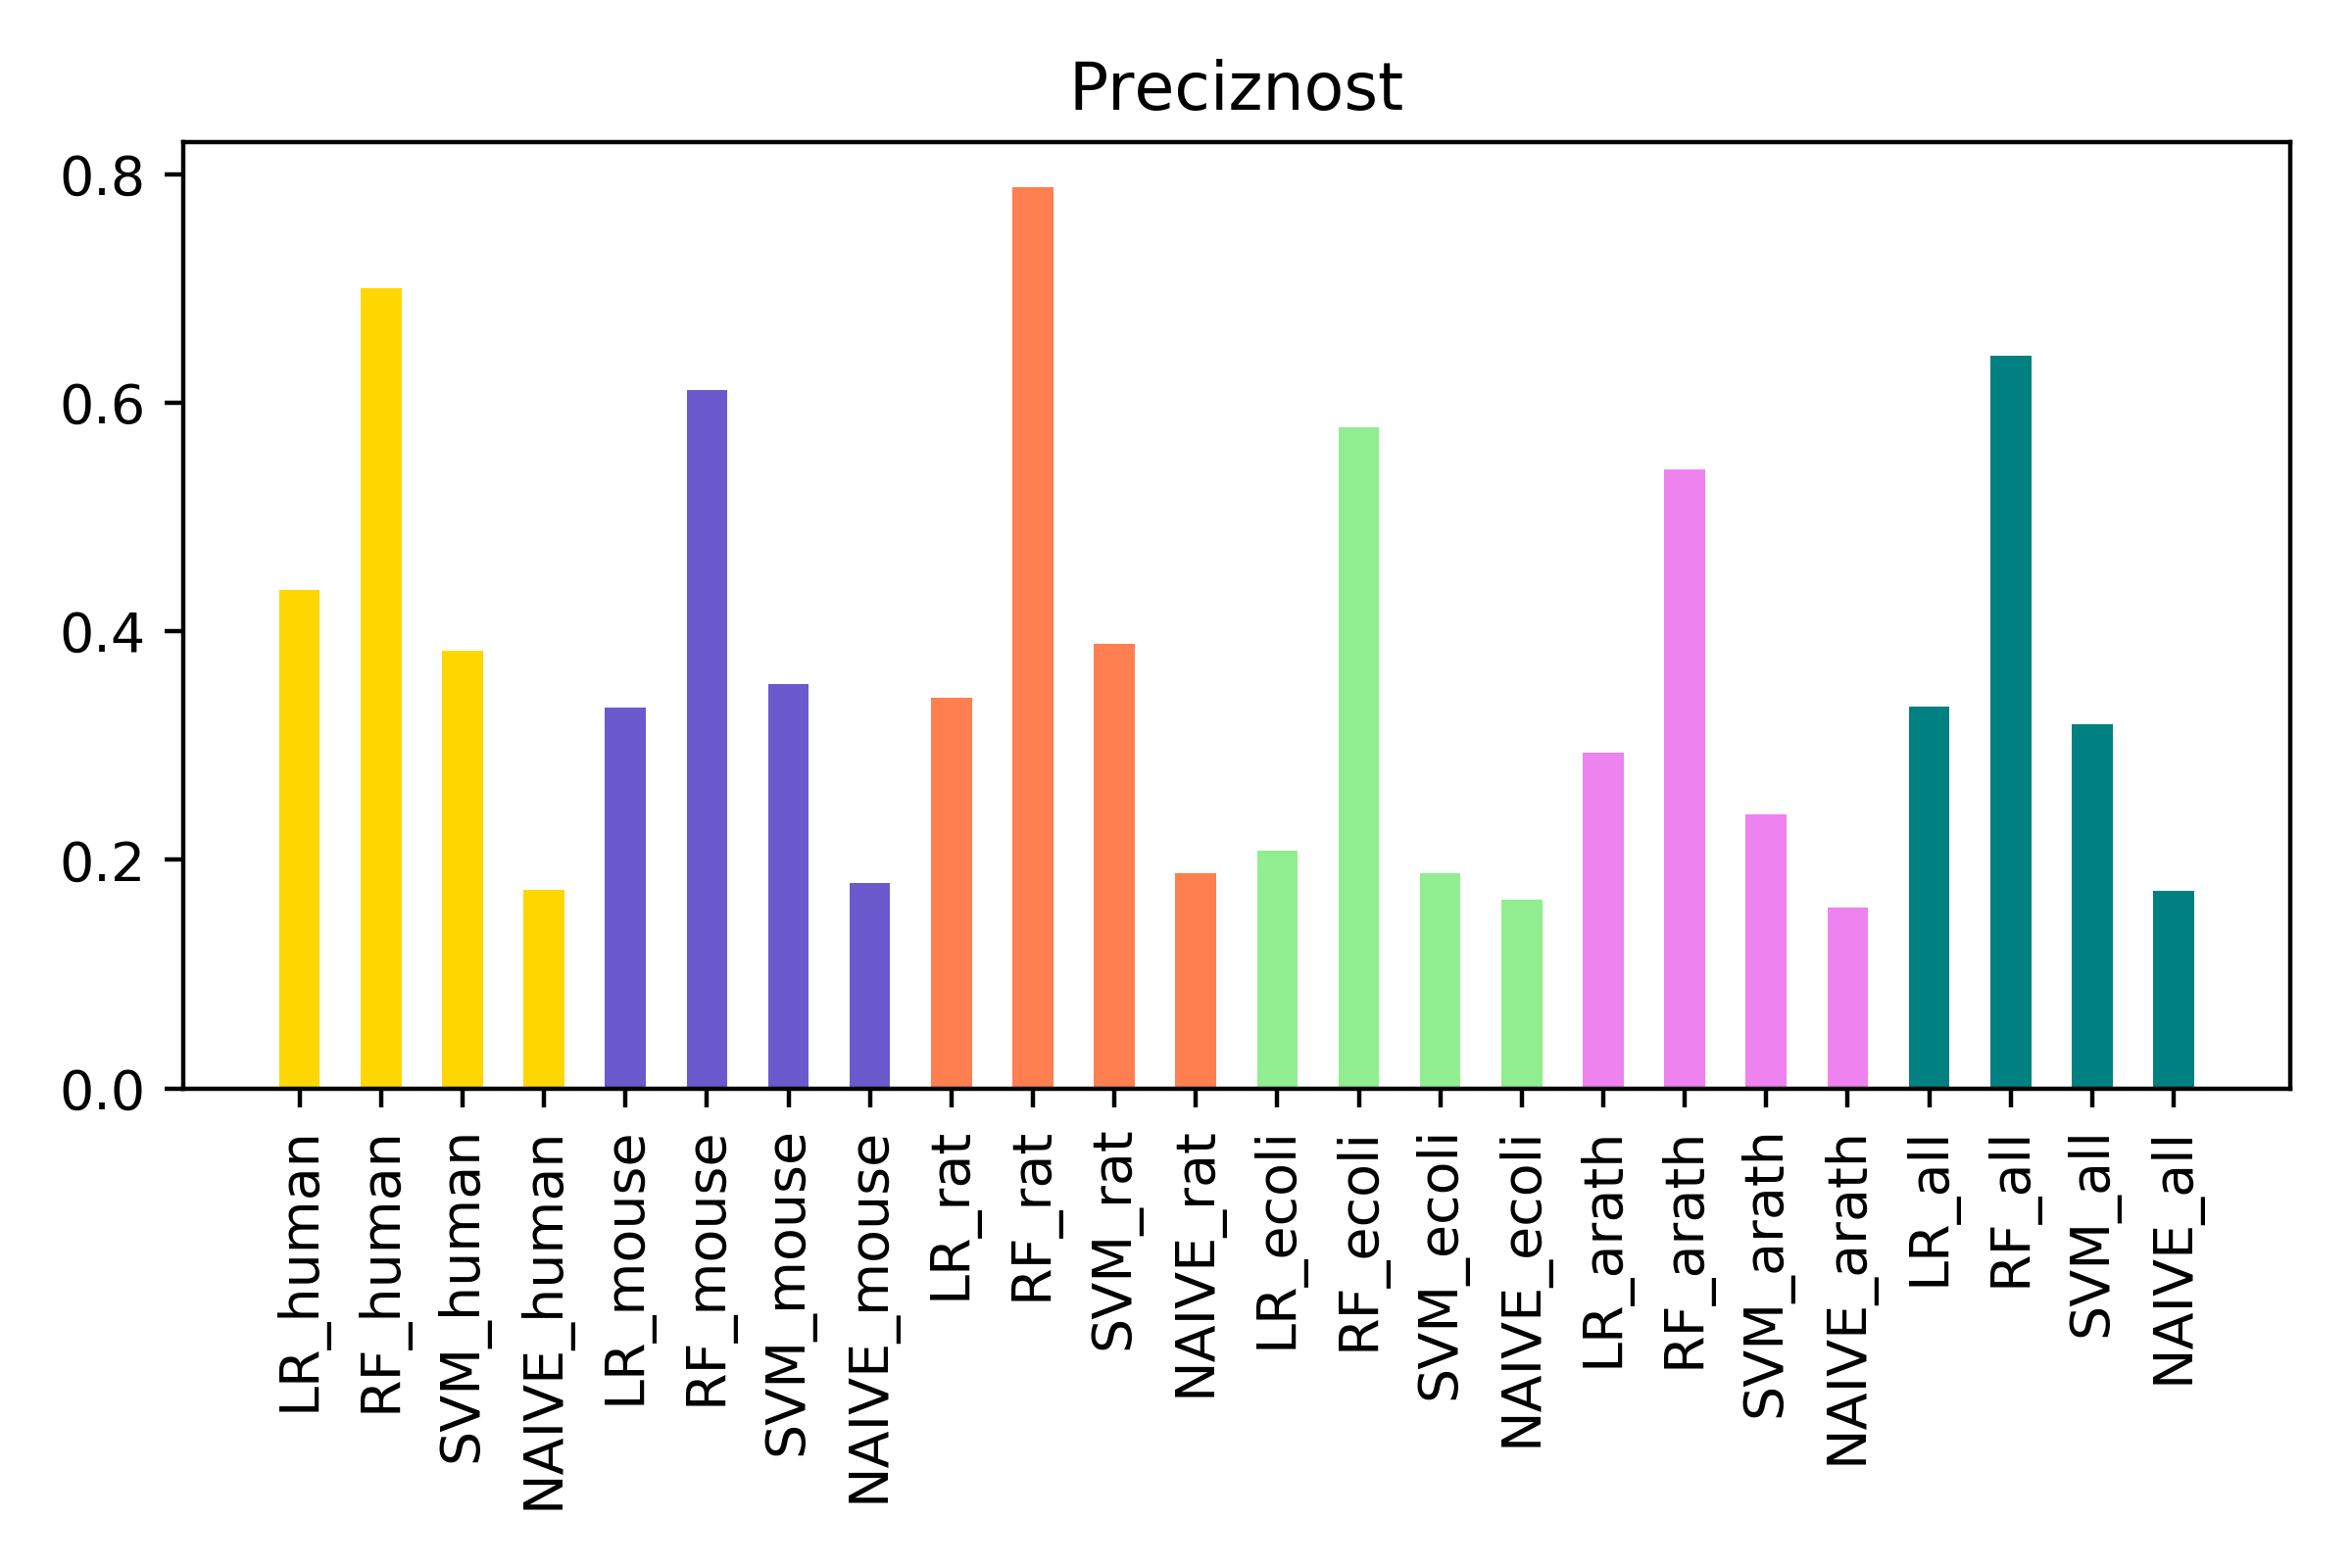
\includegraphics[width=\textwidth]{Figures/pre_poredjenje.png}
		\caption{Poređenje prema preciznosti. }
		\label{fig:prescores}
	\end{subfigure}

~
	\newline
	\newline
~

	\begin{subfigure}{0.5\textwidth}
		\centering
		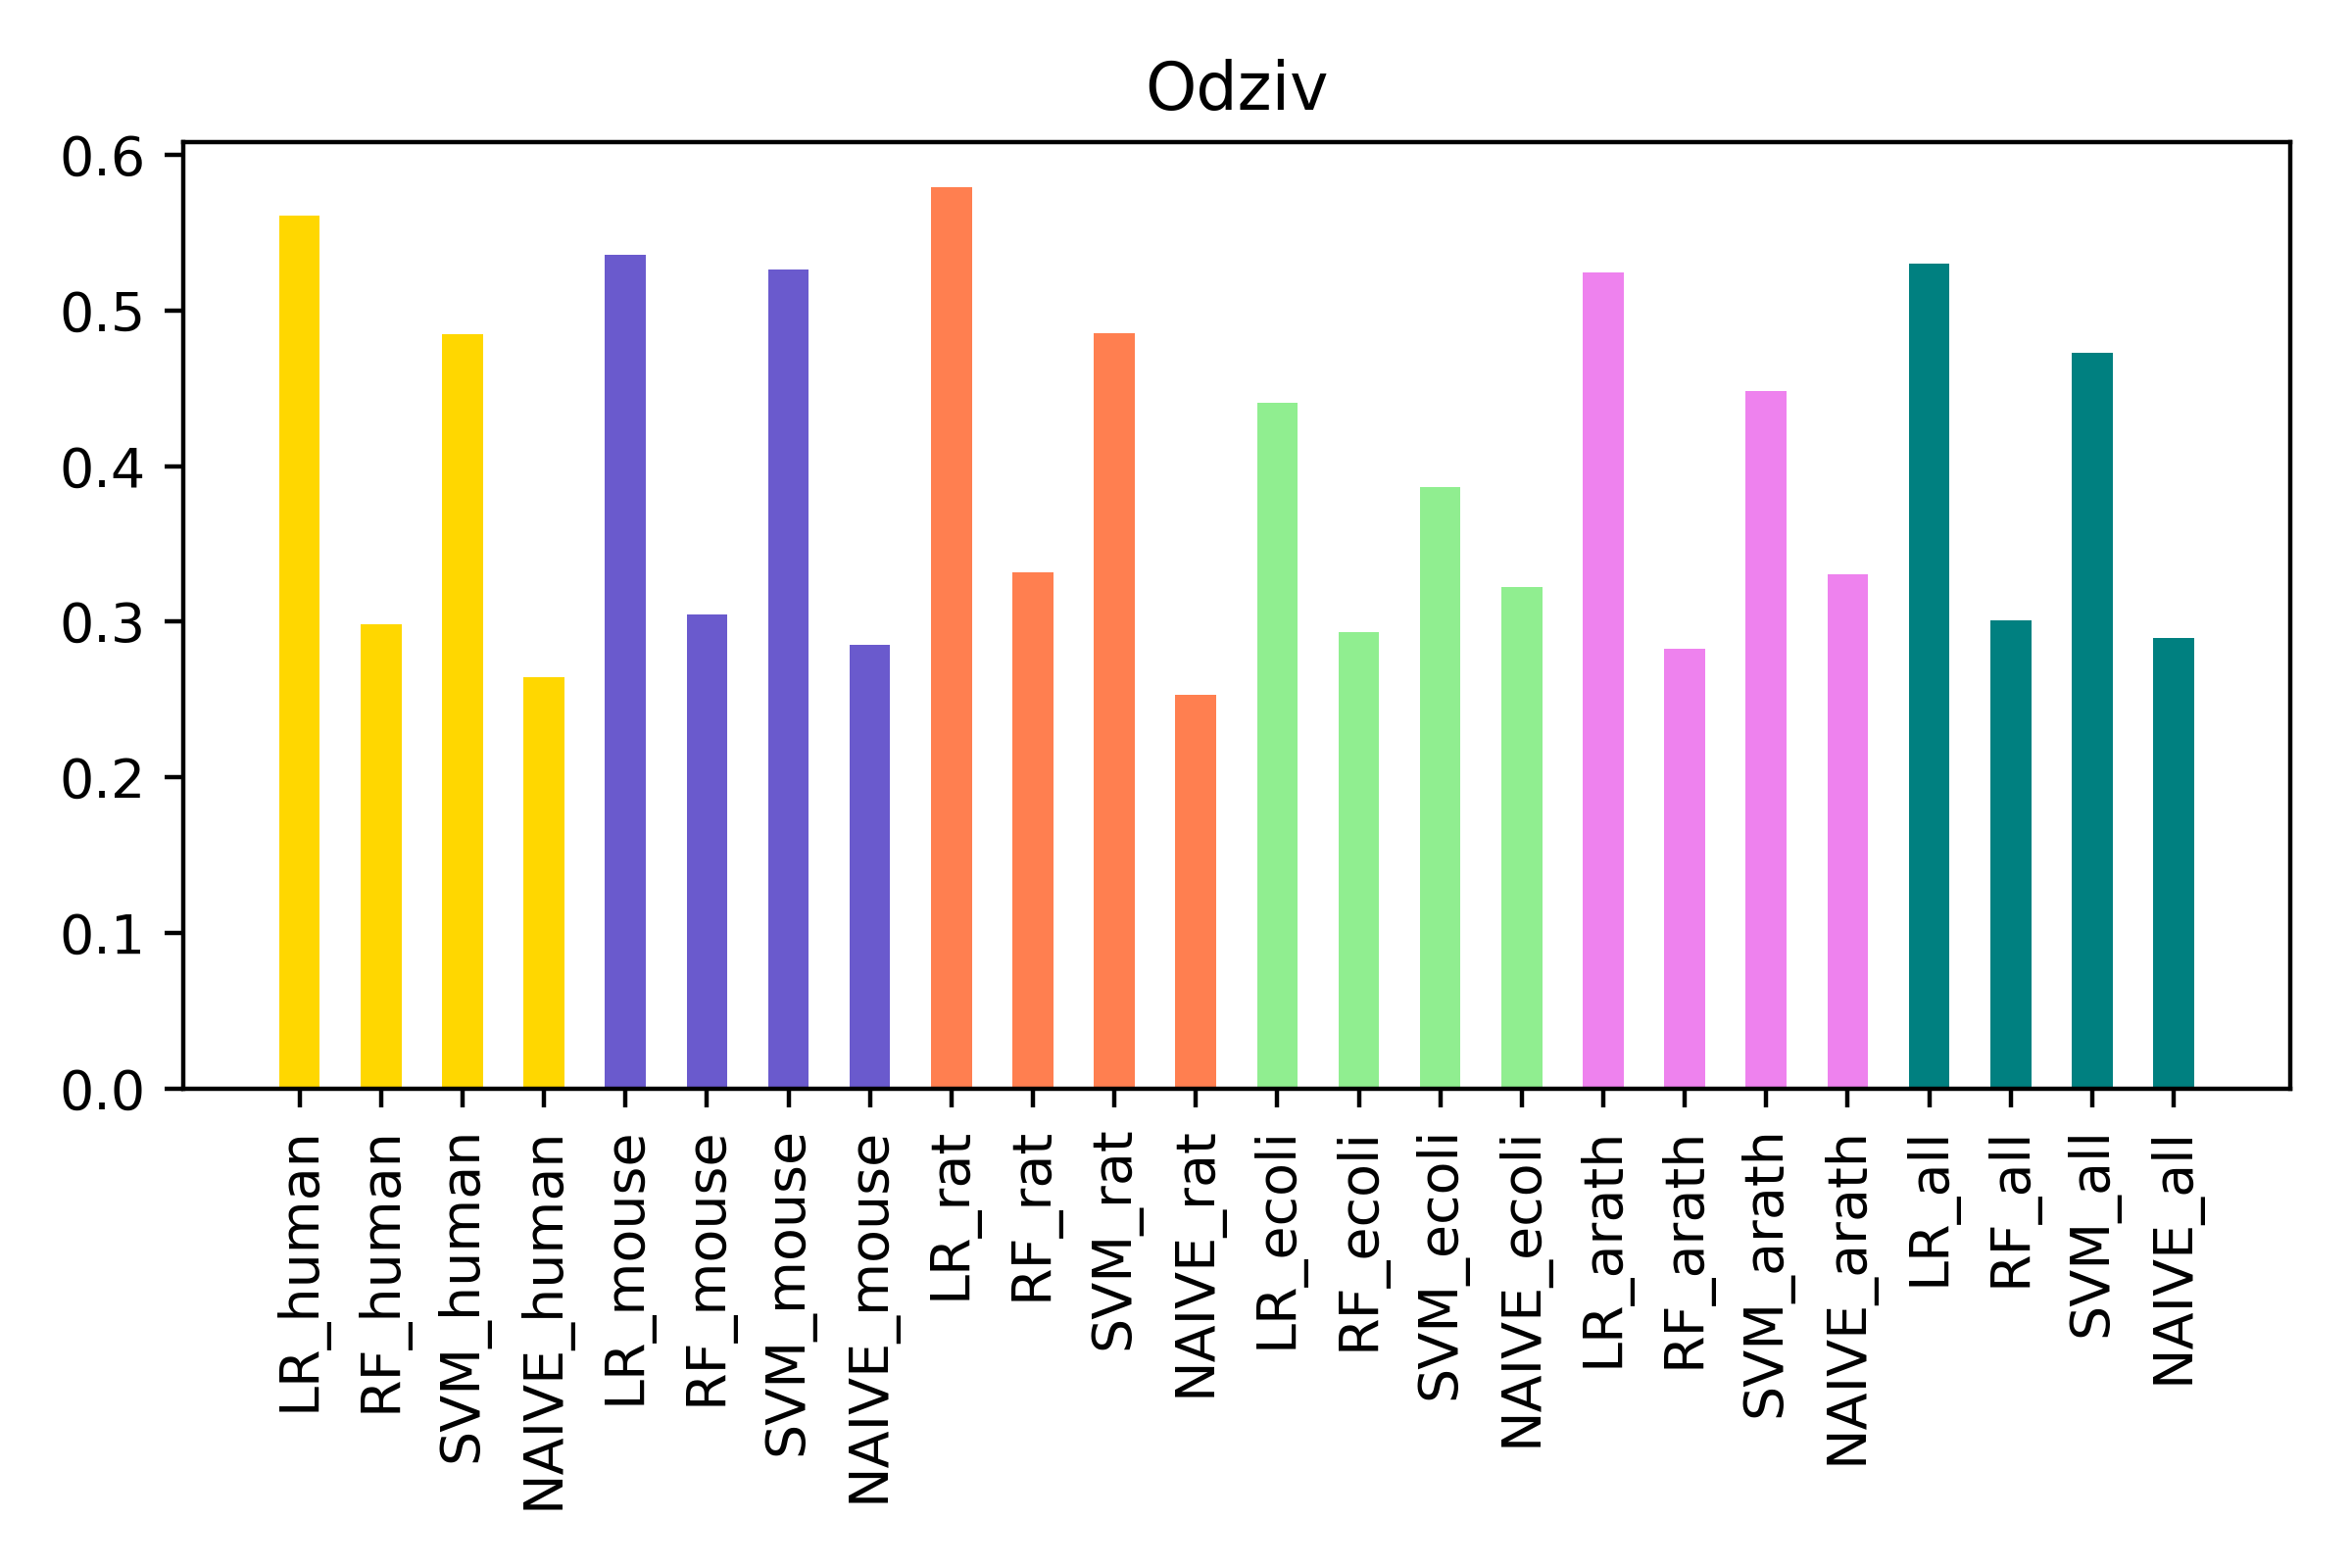
\includegraphics[width=\textwidth]{Figures/rec_poredjenje.png}
		\caption{Poređenje prema odzivu.}
		\label{fig:recscores}
	\end{subfigure}
	\begin{subfigure}{0.5\textwidth}
		\centering
		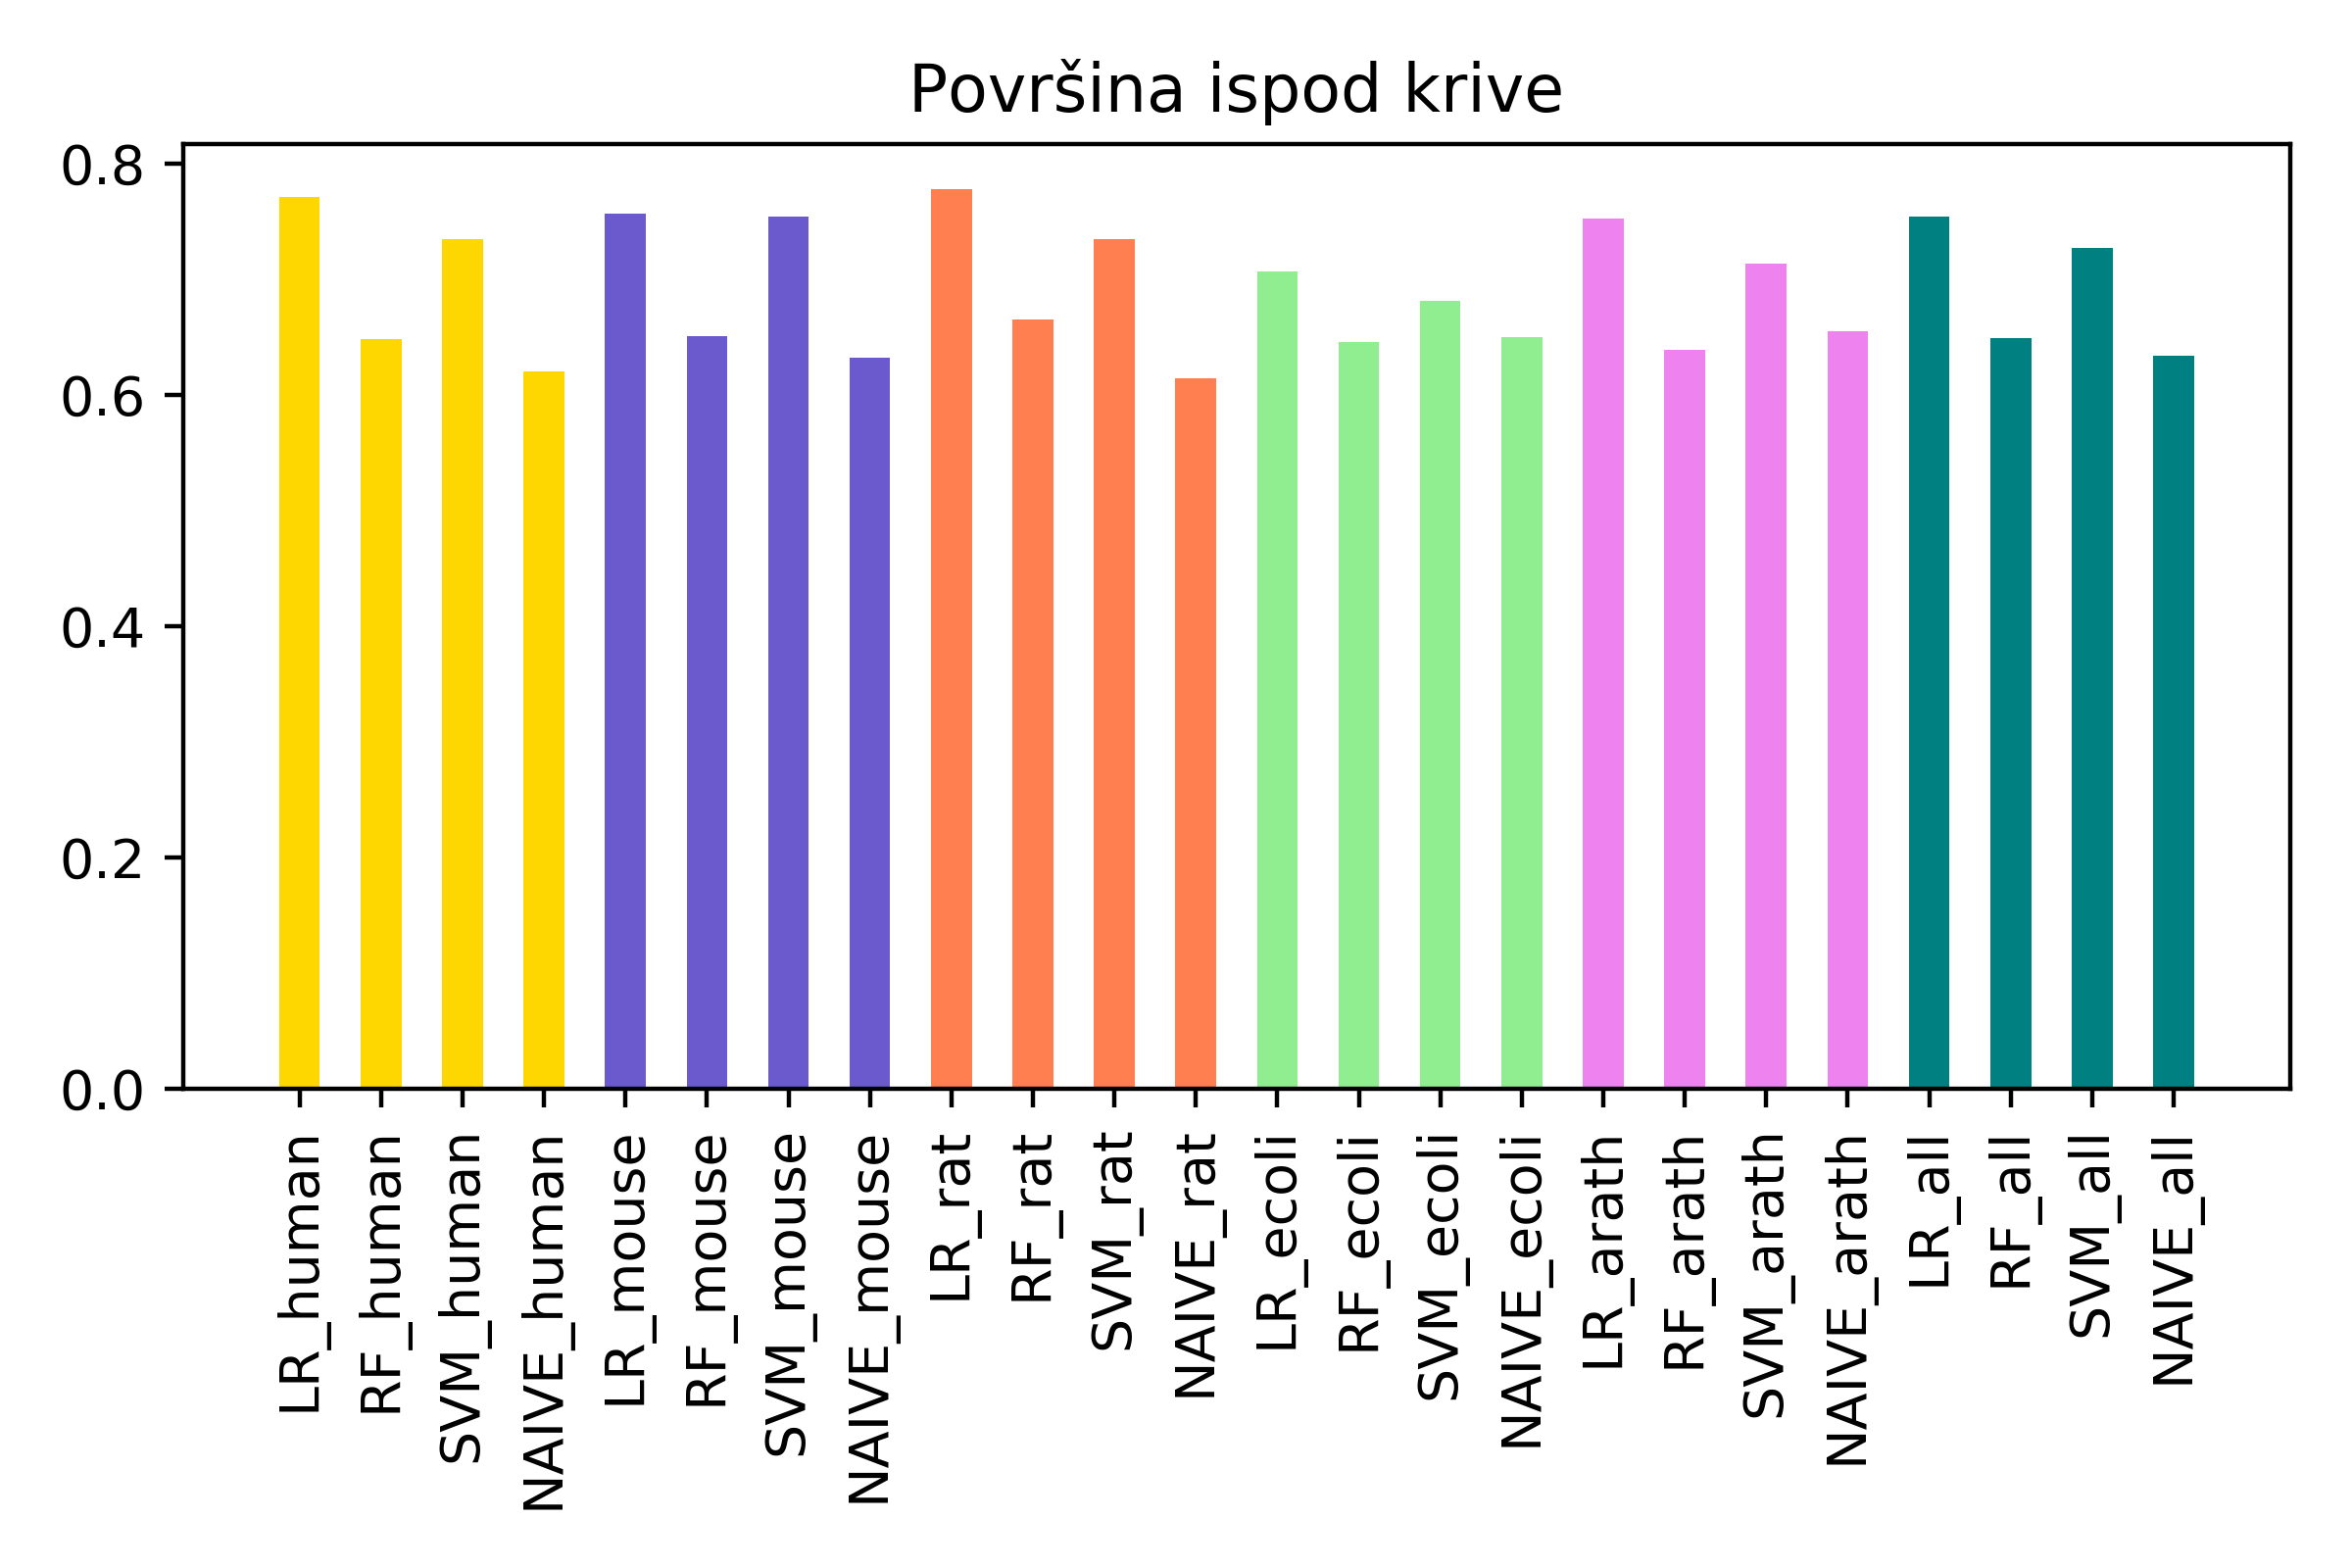
\includegraphics[width=\textwidth]{Figures/auc_poredjenje.png}
		\caption{Poređenje prema površini ispod ROC krive.}
		\label{fig:aucscores}
	\end{subfigure}
	\caption{Poređenje mera kvaliteta prediktora i naivnog klasifikatora. Rezultati jednog organizma prikazani su istom bojom.}
	\label{fig:eval}
\end{figure}

\begin{table}[h]
	\centering
	\begin{tabular}{|c|c|c|c|c|c|c|c|c|}
		\hline
		Funkcija & F1 & Acc & Pre & Rec & AUC & Nivo & Br. p. & Pr. p. \\
		\hline
		GO:0005488 & 0.84 & 0.731 & 0.74 & 0.97 & 0.54 & 1 & 15092 & 72.3\% \\
		\hline
		GO:0017171 & 0.57 & 0.991 & 0.91 & 0.42 & 0.71 & 4 & 354 & 1.7\% \\
		\hline
		GO:0016825 & 0.56 & 0.991 & 0.91 & 0.4 & 0.7 & 3 & 354 & 1.7\% \\
		\hline
		GO:0008236 & 0.54 & 0.991 & 0.93 & 0.38 & 0.69 & 5 & 349 & 1.7\% \\
		\hline
		GO:0004672 & 0.53 & 0.961 & 0.92 & 0.37 & 0.69 & 3 & 1257 & 6.0\% \\
		\hline
		GO:0003824 & 0.52 & 0.738 & 0.84 & 0.37 & 0.67 & 1 & 7843 & 37.6\% \\
		\hline
		GO:0016773 & 0.51 & 0.955 & 0.94 & 0.35 & 0.67 & 4 & 1377 & 6.6\% \\
		\hline
		GO:0016301 & 0.47 & 0.95 & 0.96 & 0.31 & 0.65 & 4 & 1452 & 7.0\% \\
		\hline
		GO:0016772 & 0.46 & 0.943 & 0.96 & 0.31 & 0.65 & 3 & 1609 & 7.7\% \\
		\hline
		GO:0004674 & 0.44 & 0.974 & 0.8 & 0.3 & 0.65 & 4 & 776 & 3.7\% \\
		\hline
		GO:0140096 & 0.42 & 0.88 & 0.89 & 0.27 & 0.63 & 2 & 3337 & 16.0\% \\
		\hline
		GO:0016740 & 0.36 & 0.881 & 0.92 & 0.23 & 0.61 & 2 & 3069 & 14.7\% \\
		\hline
		GO:0030594 & 0.32 & 0.998 & 0.75 & 0.2 & 0.6 & 3 & 86 & 0.4\% \\
		\hline
		GO:1901363 & 0.3 & 0.735 & 0.73 & 0.19 & 0.58 & 2 & 6236 & 29.9\% \\
		\hline
		GO:0016787 & 0.23 & 0.864 & 0.77 & 0.13 & 0.56 & 2 & 3202 & 15.3\% \\
		\hline
		GO:0019199 & 0.17 & 0.996 & 0.67 & 0.1 & 0.55 & 4 & 78 & 0.4\% \\
		\hline
		GO:0060089 & 0.16 & 0.957 & 0.72 & 0.09 & 0.54 & 1 & 976 & 4.7\% \\
		\hline
		GO:0038023 & 0.11 & 0.959 & 0.72 & 0.06 & 0.53 & 2 & 909 & 4.4\% \\
		\hline
		GO:0004888 & 0.11 & 0.971 & 0.75 & 0.06 & 0.53 & 3 & 626 & 3.0\% \\
		\hline
		GO:0004930 & 0.09 & 0.984 & 0.8 & 0.05 & 0.52 & 4 & 312 & 1.5\% \\
		\hline
	\end{tabular}
	\caption{Prikaz mera kvaliteta za pojedina\v cne klasifikatore metode slučajne šume za 20 \v cvorova sa najboljom $f1$-merom}
	\label{tab: rfF1}
\end{table}


Klasifikatori se odlikuju visokom preciznošću, ali niskim odzivom što znači da većinu instanci klasifikuju kao negativne, ali one koje su klasifikovane kao pozitivne su uglavnom ispravno klasifikovane. Tačnost ovih modela je visoka (oko 0.9 i više) za funckije sa manjim brojem pozitivnih instanci (ispod 10\%), dok je za funkcije sa većim brojem instanci nešto tačnost nešto manja (ispod 0.8). Slika \ref{fig:rf_ontology} ilustruje podgraf ontologije koji sadrži funkcije ove tabele.


\begin{figure}[H]
	\centering
	\includegraphics[width=\textwidth]{Figures/RFo.png}
	\caption{Prikaz podgrafa ontologije koji sadrži funkcije iz tabele \ref{tab: rfF1}}
	\label{fig:rf_ontology}
\end{figure}

\begin{table}[h]
	\centering
	\begin{tabular}{|c|c|c|c|c|c|c|c|c|}
		\hline
		Funkcija & F1 & Acc & Pre & Rec & AUC & Nivo & Br. p. & Pr. p. \\
		\hline
		GO:0004672 & 0.82 & 0.979 & 0.82 & 0.81 & 0.9 & 3 & 1257 & 6.0\% \\
		\hline
		GO:0004930 & 0.79 & 0.993 & 0.84 & 0.74 & 0.87 & 4 & 312 & 1.5\% \\
		\hline
		GO:0016773 & 0.77 & 0.97 & 0.78 & 0.75 & 0.87 & 4 & 1377 & 6.6\% \\
		\hline
		GO:0005488 & 0.76 & 0.673 & 0.8 & 0.73 & 0.63 & 1 & 15092 & 72.3\% \\
		\hline
		GO:0004674 & 0.74 & 0.98 & 0.65 & 0.87 & 0.93 & 4 & 776 & 3.7\% \\
		\hline
		GO:0016301 & 0.73 & 0.961 & 0.72 & 0.74 & 0.86 & 4 & 1452 & 7.0\% \\
		\hline
		GO:0003824 & 0.71 & 0.756 & 0.65 & 0.77 & 0.76 & 1 & 7843 & 37.6\% \\
		\hline
		GO:0008236 & 0.7 & 0.992 & 0.71 & 0.69 & 0.84 & 5 & 349 & 1.7\% \\
		\hline
		GO:0016825 & 0.69 & 0.991 & 0.68 & 0.71 & 0.85 & 3 & 354 & 1.7\% \\
		\hline
		GO:0017171 & 0.69 & 0.991 & 0.69 & 0.68 & 0.84 & 4 & 354 & 1.7\% \\
		\hline
		GO:0016772 & 0.67 & 0.948 & 0.69 & 0.64 & 0.81 & 3 & 1609 & 7.7\% \\
		\hline
		GO:0030594 & 0.63 & 0.997 & 0.52 & 0.8 & 0.9 & 3 & 86 & 0.4\% \\
		\hline
		GO:0004888 & 0.61 & 0.972 & 0.52 & 0.75 & 0.87 & 3 & 626 & 3.0\% \\
		\hline
		GO:0019199 & 0.61 & 0.996 & 0.52 & 0.75 & 0.87 & 4 & 78 & 0.4\% \\
		\hline
		GO:0140096 & 0.59 & 0.858 & 0.54 & 0.65 & 0.78 & 2 & 3337 & 16.0\% \\
		\hline
		GO:0038023 & 0.58 & 0.964 & 0.58 & 0.59 & 0.78 & 2 & 909 & 4.4\% \\
		\hline
		GO:0060089 & 0.58 & 0.96 & 0.55 & 0.61 & 0.79 & 1 & 976 & 4.7\% \\
		\hline
		GO:1901363 & 0.56 & 0.703 & 0.5 & 0.64 & 0.69 & 2 & 6236 & 29.9\% \\
		\hline
		GO:0016740 & 0.53 & 0.844 & 0.49 & 0.58 & 0.74 & 2 & 3069 & 14.7\% \\
		\hline
		GO:0016787 & 0.46 & 0.808 & 0.4 & 0.55 & 0.7 & 2 & 3202 & 15.3\% \\
		\hline
	\end{tabular}
	\caption{Prikaz mera kvaliteta za pojedina\v cne klasifikatore metode logistička regresija  za 20 \v cvorova sa najboljom $f1$-merom}
	\label{tab: lrF1}
\end{table}

~\\ 
Najbolji modeli logističke regresije odlikuju se približnim merama za preciznost i odziv. Tačnost modela je veća kod modela sa manjim brojem pozitivnih instanci kao i kod metode slučajnih šuma.

\begin{figure}[H]
	\centering
	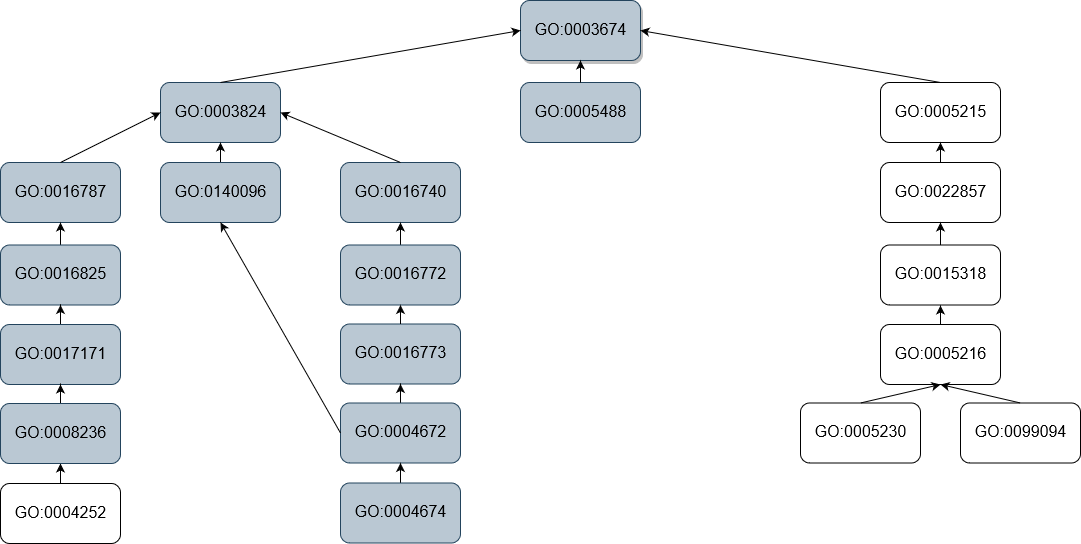
\includegraphics[width=\textwidth]{Figures/LRo.png}
	\caption{Prikaz podgrafa ontologije koji sadrži funkcije iz tabele \ref{tab: lrF1}}
	\label{fig:lr_ontology}
\end{figure}

\begin{table}[h]
	\centering
	\begin{tabular}{|c|c|c|c|c|c|c|c|c|}
		\hline
		Funkcija & F1 & Acc & Pre & Rec & AUC & Nivo & Br. p. & Pr. p. \\
		\hline
		GO:0004672 & 0.81 & 0.978 & 0.84 & 0.78 & 0.88 & 3 & 1257 & 6.0\% \\
		\hline
		GO:0030594 & 0.79 & 0.999 & 0.85 & 0.73 & 0.87 & 3 & 86 & 0.4\% \\
		\hline
		GO:0004930 & 0.78 & 0.992 & 0.73 & 0.84 & 0.92 & 4 & 312 & 1.5\% \\
		\hline
		GO:0005488 & 0.78 & 0.696 & 0.81 & 0.75 & 0.65 & 1 & 15092 & 72.3\% \\
		\hline
		GO:0016773 & 0.76 & 0.97 & 0.81 & 0.72 & 0.85 & 4 & 1377 & 6.6\% \\
		\hline
		GO:0004674 & 0.75 & 0.981 & 0.67 & 0.86 & 0.92 & 4 & 776 & 3.7\% \\
		\hline
		GO:0016301 & 0.75 & 0.967 & 0.82 & 0.68 & 0.84 & 4 & 1452 & 7.0\% \\
		\hline
		GO:0003824 & 0.72 & 0.786 & 0.71 & 0.74 & 0.78 & 1 & 7843 & 37.6\% \\
		\hline
		GO:0019199 & 0.72 & 0.998 & 0.74 & 0.7 & 0.85 & 4 & 78 & 0.4\% \\
		\hline
		GO:0017171 & 0.71 & 0.991 & 0.65 & 0.78 & 0.89 & 4 & 354 & 1.7\% \\
		\hline
		GO:0016825 & 0.71 & 0.992 & 0.75 & 0.67 & 0.83 & 3 & 354 & 1.7\% \\
		\hline
		GO:0008236 & 0.7 & 0.991 & 0.64 & 0.76 & 0.88 & 5 & 349 & 1.7\% \\
		\hline
		GO:0016772 & 0.67 & 0.951 & 0.73 & 0.62 & 0.8 & 3 & 1609 & 7.7\% \\
		\hline
		GO:0004888 & 0.64 & 0.98 & 0.68 & 0.6 & 0.8 & 3 & 626 & 3.0\% \\
		\hline
		GO:0038023 & 0.63 & 0.971 & 0.69 & 0.57 & 0.78 & 2 & 909 & 4.4\% \\
		\hline
		GO:0060089 & 0.62 & 0.967 & 0.66 & 0.59 & 0.79 & 1 & 976 & 4.7\% \\
		\hline
		GO:0140096 & 0.59 & 0.883 & 0.66 & 0.54 & 0.75 & 2 & 3337 & 16.0\% \\
		\hline
		GO:1901363 & 0.57 & 0.728 & 0.54 & 0.61 & 0.69 & 2 & 6236 & 29.9\% \\
		\hline
		GO:0016740 & 0.55 & 0.873 & 0.59 & 0.51 & 0.72 & 2 & 3069 & 14.7\% \\
		\hline
		GO:0016787 & 0.48 & 0.842 & 0.48 & 0.49 & 0.7 & 2 & 3202 & 15.3\% \\
		\hline
	\end{tabular}
	\caption{Prikaz mera kvaliteta za pojedina\v cne klasifikatore metode potpornih vektora za 20 \v cvorova sa najboljom $f1$-merom}
	\label{tab: svmF1}
\end{table}


~\\
~\\

Najbolji modeli metode potpornih vektora pokazuju slično ponašanje kao modeli logističke regresije.

~\\

\begin{figure}[H]
	\centering
	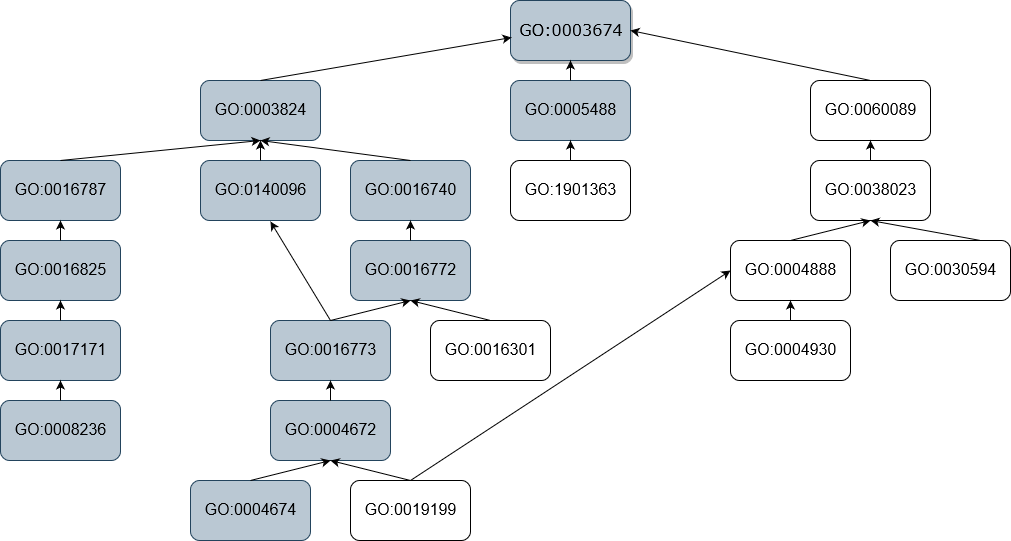
\includegraphics[width=\textwidth]{Figures/SVMo.png}
	\caption{Prikaz podgrafa ontologije koji sadrži funkcije iz tabele \ref{tab: svmF1}}
	\label{fig:svm_ontology}
\end{figure}

\newpage

Prikazani podgrafi sadrže zajedničke čvorove odnosno, sva tri prediktora su za nekoliko istih funkcija dali najbolje rezultate. Nazivi ovih funckija navedeni su u tabeli \ref{tab: commonNames}. Poređenje mera kvaliteta klasifikatora ovih funkcija prikazano je u tabeli \ref{tab: commonScores}, a na slikama su zajednički čvorovi označeni sivom bojom.

~\\

\begin{table}[H]
	\centering
	\begin{tabular}{|c|l|}
		\hline
		Oznaka funkcije & Naziv funkcije \\
		\hline
		GO:0003674 & molecular\_function\\
		\hline
		GO:0003824 & catalytic activity\\
		\hline
		GO:0005488 & binding\\
		\hline
		GO:0016787 & hydrolase activity\\
		\hline
		GO:0140096 & catalytic activity, acting on a protein\\
		\hline
		GO:0016740 & transferase activity\\
		\hline
		GO:0016825 & hydrolase activity, acting on acid phosphorus-nitrogen bonds \\
		\hline
		GO:0016772 & transferase activity, transferring phosphorus-containing groups\\
		\hline
		GO:0017171 & serine hydrolase activity \\
		\hline
		GO:0016773 & phosphotransferase activity, alcohol group as acceptor \\
		\hline
		GO:0008236 & serine-type peptidase activity \\
		\hline
		GO:0004672 & protein kinase activity \\
		\hline
		GO:0004674 & protein serine/threonine kinase activity \\
		\hline
	\end{tabular}
	\caption{Oznake i nazivi funkcija za zajedničke čvorove podgrafa sa slika \ref{fig:rf_ontology}, \ref{fig:lr_ontology} i \ref{fig:svm_ontology}} 
	\label{tab: commonNames}
\end{table}


~\\

Modeli metode slučajnih šuma za iste funkcije daju nešto slabiju $f1$-meru u poređenju sa ostalim metodama, ali zato je preciznost skoro svih modela veća u odnosu na modele drugih metoda. Tačnost svih modela su prilično bliske, dok se prema odzivu najviše ističu modeli linearne regresije. Površina ispod ROC krive je slična za modele logističke regresije i modela potpornih vektora, a slučajne šume su dale nešto slabije rezultate.



\begin{landscape}
\begin{table}[H]
	\centering
	\begin{tabular}{V{3.5}cV{3.5}c|c|cV{3.5}c|c|cV{3.5}c|c|cV{3.5}c|c|cV{3.5}c|c|cV{3.5}}
		\hlineB{3.5}
		\multirow{3}{*}{Oznaka funkcije} & \multicolumn{3}{cV{3.5}}{\multirow{2}{*}{F1-mera}} & \multicolumn{3}{cV{3.5}}{\multirow{2}{*}{Ta\v cnost}}  & \multicolumn{3}{cV{3.5}}{\multirow{2}{*}{Preciznost}} & \multicolumn{3}{cV{3.5}}{\multirow{2}{*}{Odziv}}  & \multicolumn{3}{cV{3.5}}{Povr\v sina ispod} \\
		& \multicolumn{3}{cV{3.5}}{} & \multicolumn{3}{cV{3.5}}{} & \multicolumn{3}{cV{3.5}}{} & \multicolumn{3}{cV{3.5}}{} & \multicolumn{3}{cV{3.5}}{ROC krive} \\
		\cline{2-16}
		& LR & RF & SVM & LR & RF & SVM & LR & RF & SVM & LR & RF & SVM & LR & RF & SVM \\
		\hlineB{3.5}
		GO:0003824 & 0.71 & 0.52 & \textbf{0.72} &0.76 & 0.74 & \textbf{0.79} &0.65 & \textbf{0.84} & 0.71 & \textbf{0.77} & 0.37 & 0.74 &0.76 & 0.67 & \textbf{0.78}\\
		\hline
		GO:0005488 & 0.76 & \textbf{0.84} & 0.78 & 0.67 & \textbf{0.73} & 0.7 & 0.8 & 0.74 & \textbf{0.81} & 0.73 & \textbf{0.97} & 0.75 & 0.63 & 0.54 & \textbf{0.65}\\
		\hline
		GO:0016787 & 0.46 & 0.23 & \textbf{0.48} & 0.81 & \textbf{0.86} & 0.84 & 0.4 & \textbf{0.77} & 0.48 & \textbf{0.55} & 0.13 & 0.49 & \textbf{0.7} & 0.56 & \textbf{0.7}\\
		\hline
		GO:0140096 & \textbf{0.59} & 0.42 & \textbf{0.59} & 0.86 & \textbf{0.88} & \textbf{0.88} &0.54 & \textbf{0.89} & 0.66 & \textbf{0.65} & 0.27 & 0.54 & \textbf{0.78} & 0.63 & 0.75\\
		\hline
		GO:0016740 & 0.53 & 0.36 & \textbf{0.55} & 0.84 & \textbf{0.88} & 0.87 & 0.49 & \textbf{0.92} & 0.59 & \textbf{0.58} & 0.23 & 0.51 & \textbf{0.74} & 0.61 & 0.72\\
		\hline
		GO:0016825 & 0.69 & 0.56 & \textbf{0.71} & \textbf{0.99} & \textbf{0.99} & \textbf{0.99} & 0.68 & \textbf{0.91} & 0.75 & \textbf{0.71} & 0.4 & 0.67 & \textbf{0.85} & 0.7 & 0.83\\
		\hline
		GO:0016772 & \textbf{0.67} & 0.46 & \textbf{0.67} & \textbf{0.95} & 0.94 & \textbf{0.95} & 0.69 & \textbf{0.96} & 0.73 & \textbf{0.64} & 0.31 & 0.62 & \textbf{0.81} & 0.65 & 0.8\\
		\hline
		GO:0017171 & 0.69 & 0.57 & \textbf{0.71} & \textbf{0.99} & \textbf{0.99} & \textbf{0.99} & 0.69 & \textbf{0.91} & 0.65 & 0.68 & 0.42 & \textbf{0.78} & 0.84 & 0.71 & \textbf{0.89}\\
		\hline
		GO:0016773 & \textbf{0.77} & 0.51 & 0.76 & \textbf{0.97} & 0.96 & \textbf{0.97} & 0.78 & \textbf{0.94} & 0.81 & \textbf{0.75} & 0.35 & 0.72 & \textbf{0.87} & 0.67 & 0.85\\
		\hline
		GO:0008236 & \textbf{0.7} & 0.54 & \textbf{0.7} & \textbf{0.99} & \textbf{0.99} & \textbf{0.99} & 0.71 & \textbf{0.93} & 0.64 & 0.69 & 0.38 & \textbf{0.76} & 0.84 & 0.69 & \textbf{0.88}\\
		\hline
		GO:0004672 & \textbf{0.82} & 0.53 & 0.81 & \textbf{0.98} & 0.96 & \textbf{0.98} & 0.82 & \textbf{0.92} & 0.84 & \textbf{0.81} & 0.37 & 0.78 & \textbf{0.9} & 0.69 & 0.88\\
		\hline
		GO:0004674 & 0.74 & 0.44 & \textbf{0.75} & \textbf{0.98} & 0.97 & \textbf{0.98} & 0.65 & \textbf{0.8} & 0.67 & \textbf{0.87} & 0.3 & 0.86 & \textbf{0.93} & 0.65 & 0.92\\
		\hlineB{3.5}
	\end{tabular}
	\caption{Pore\dj enje mera kvaliteta za zajedni\v cke \v cvorove podgrafa sa slika \ref{fig:rf_ontology}, \ref{fig:lr_ontology} i \ref{fig:svm_ontology}} 
	\label{tab: commonScores}
	\end{table}
	
\end{landscape}

Predikotri su dodatno testirani na \textit{benchmark} skupu proteina koji je korišćen u okviru CAFA3 takmičenja \cite{biofCafa}. Skup sadrži 453 proteina različitih organizama. Izračunata je prosečna vrednost $f_1$-mera za svaki prediktor, a dobijeni rezultati su dodatno upoređeni sa rezultatima učesnika takmičenja \cite{cafa}. 

Prediktor za metodu slučajnih šuma dao je najbolji rezultat od tri prediktora, čime je među učesnicima ovog takmičenja zauzeo 85. mesto među 136 tačkmičara. Poređenje sva tri prediktora sa svim učesnicima prikazano je na slici \ref{fig:cafa}.


\begin{figure}[H]
	\centering
	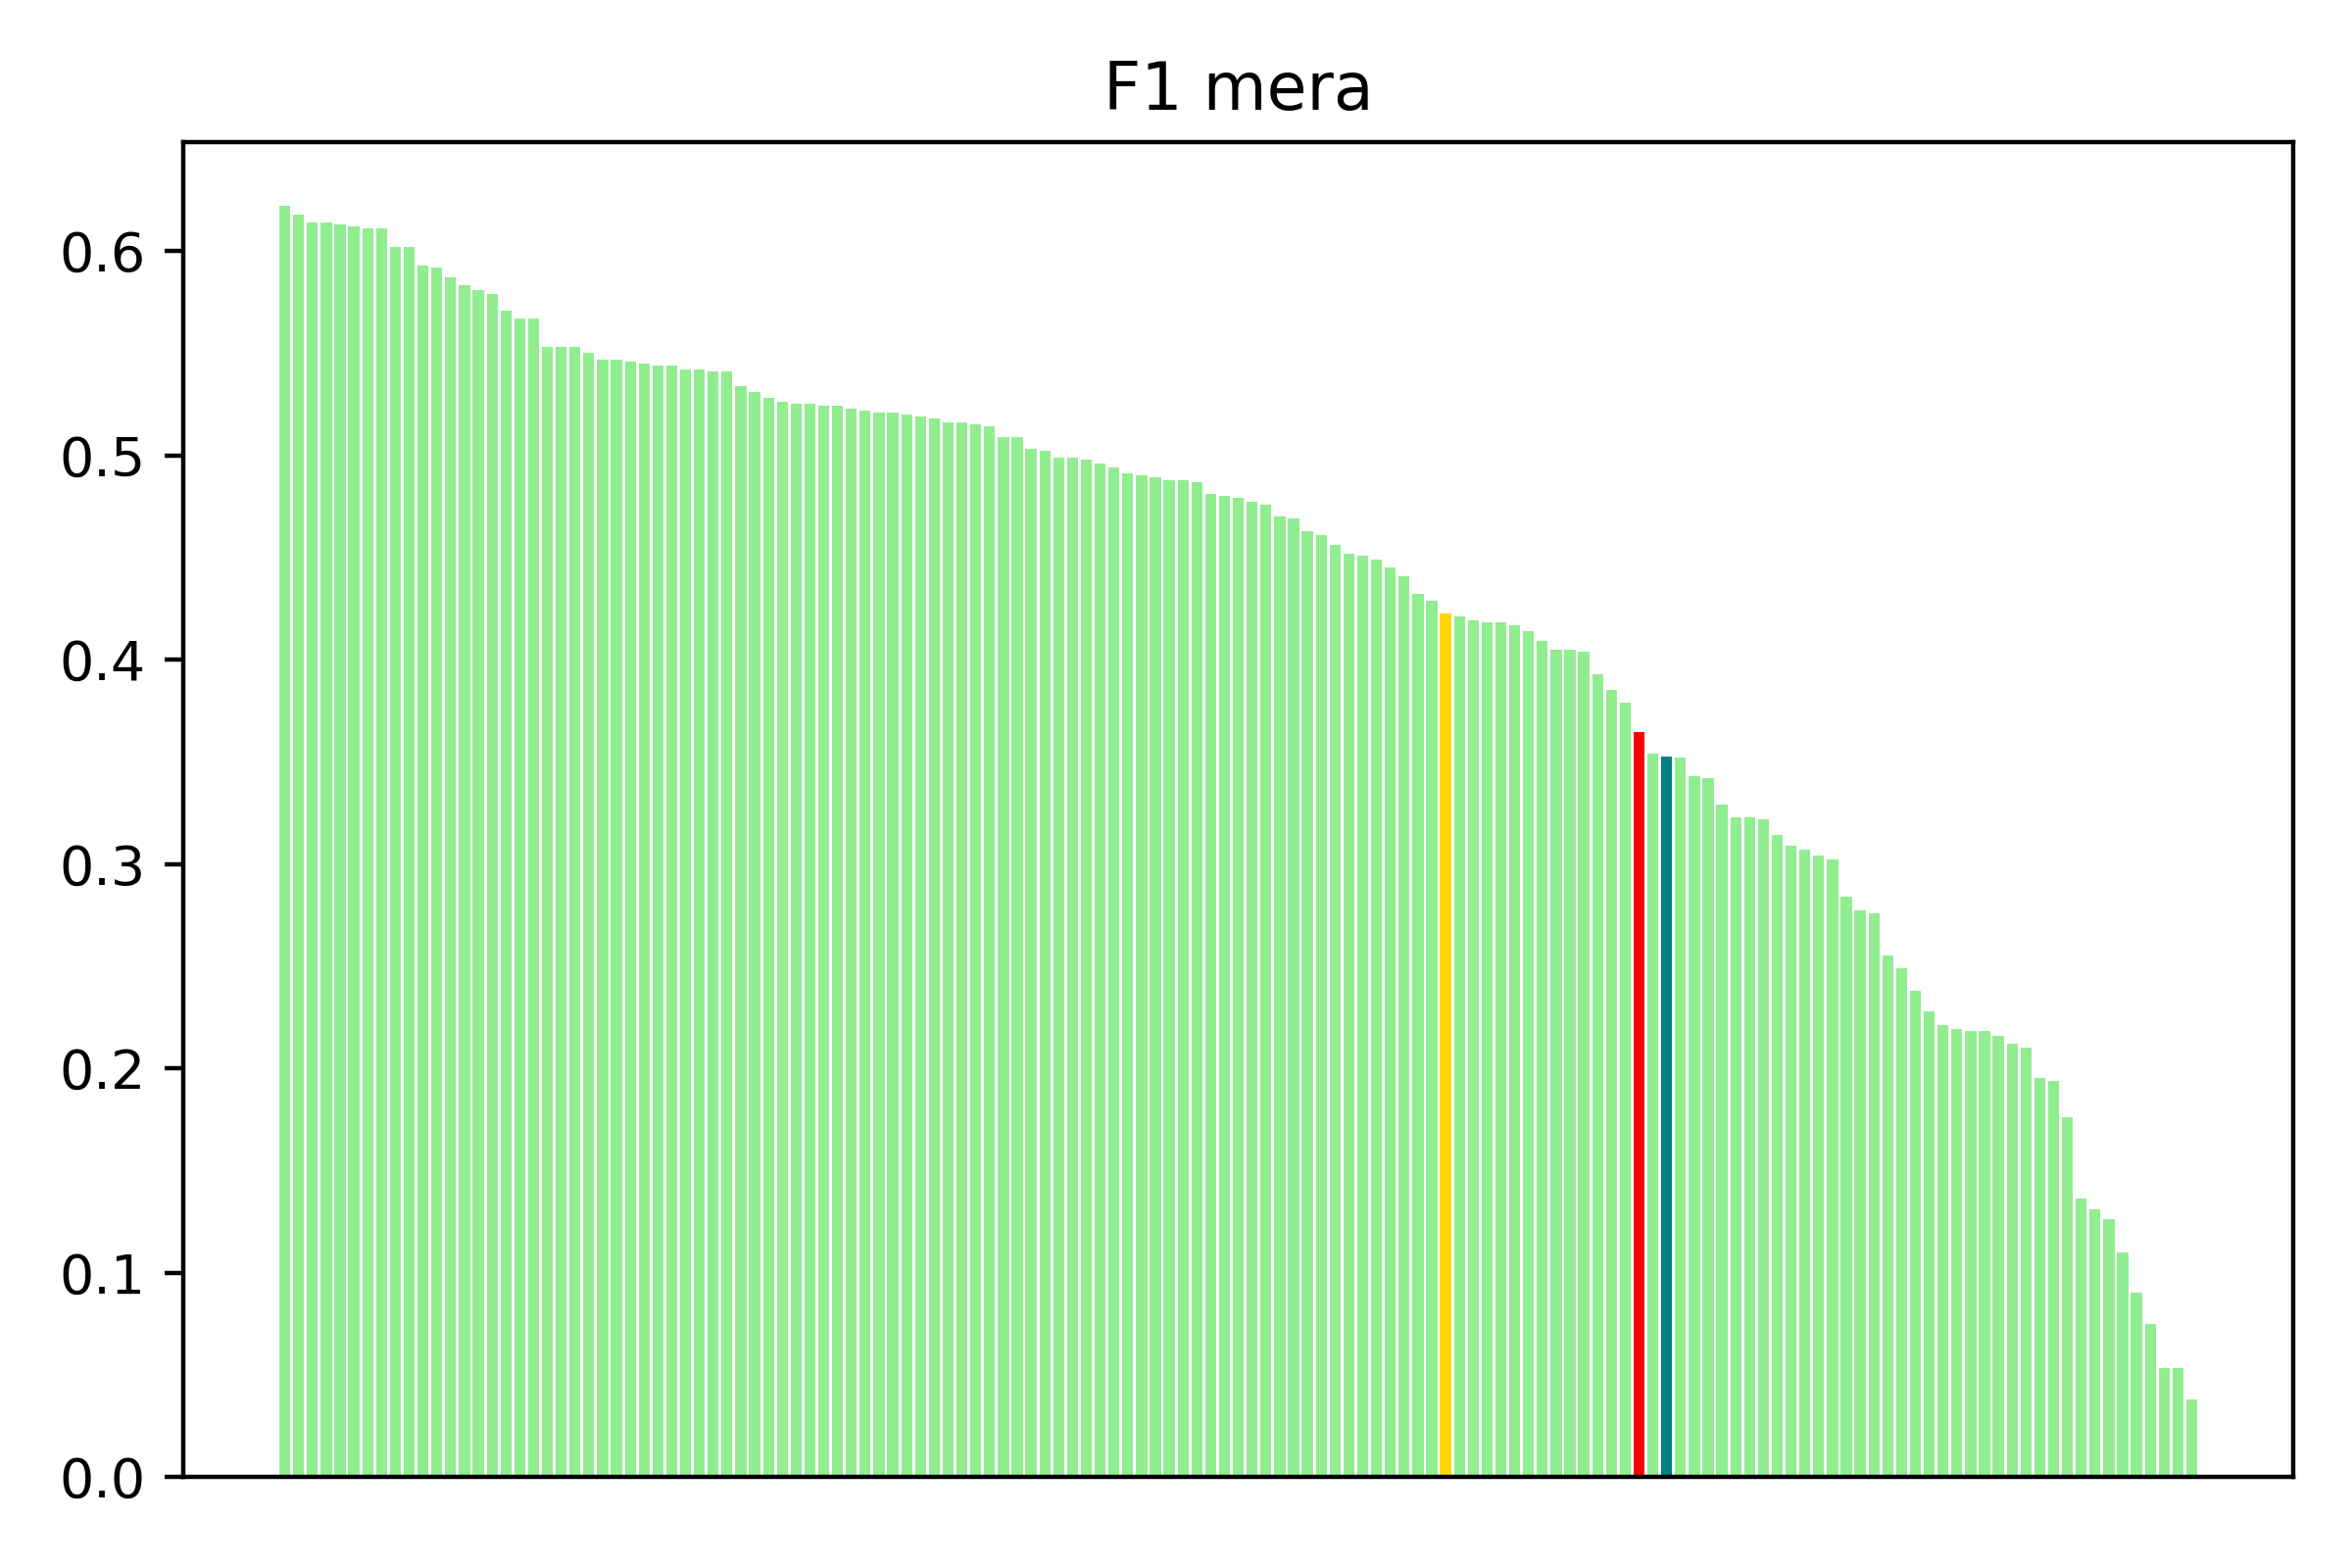
\includegraphics[width=\textwidth]{Figures/cafa_poredjenje.png}
	\caption{Poređenje $f_1$-mera tri prediktora sa rezultatima učesnika  CAFA3 takmičenja. Crvenom bojom označen je prediktor linearne regresije, žutom prediktor slučajnih šuma, plavom prediktor metode potpornih vektora. Svetlo zelenom bojom prikazani su rezultati postignuti na CAFA3 takmičenju.}
	\label{fig:cafa}
\end{figure}


